% Chapter 1
\setstretch{1.8}

\chapter{Literature Study of Induction Motors} % Write in your own chapter title
\label{Literature Study of Induction Motors}
\lhead{Chapter 2. \emph{Literature Study of Induction Motors}} % Write in your own chapter title to set the page header

\section{Induction motors}
In Present times, induction motors are the workhorse of the modern industry. They the most used type of electric machine in the industry as well as domestic use, since they are relatively low-cost and robust. Additionally, they are even appropriate for inflammable work environments such as sawmills and chemical factories\cite{esenozdemir2016}. Particularly, the advancement of the converter technology has enabled quite accurate control of the induction motors. Therefore, making it possible to use induction motors even in applications which involve accurate speed control. This section describes the working principles, structures and steady state equivalent circuit of an induction motor.

\section{Induction motor structure}
There are two main types of induction motors: 
\begin{itemize}
	\item Wound rotor induction motor 
	\item Squirrel Cage induction motor. 
\end{itemize}

This chapter focuses only on the latter one, because the test bench was implemented with a Squirrel Cage type induction motor. The assembly of a Squirrel cage induction motor consists of two major parts which are:
\begin{itemize}
	\item Stator winding 
	\item Rotor cage
\end{itemize}

These parts are shown in Figure 1 where portion of the induction motor body and stator has been cut. This exposes the laminated cage rotor mounted to the shaft and stator winding near it. Moreover, supplementary structures are added to the design of motor from time to time so as to gain some desired features depending on the application
\begin{figure}[htbp]
	\centering
		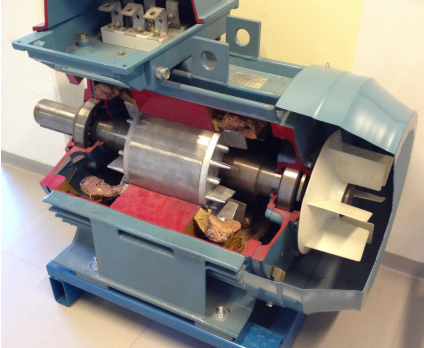
\includegraphics[width = 4.5in]{./Figures/MS/26.png}
		\rule{35em}{0.5pt}
	\caption{Cut-out of a squirrel cage induction motor}
	\label{fig:Cut-out of a squirrel cage induction motor}
\end{figure}

The cage rotor consists of bars constructed from a conductive substance. Typically, they are created from aluminum or copper and both sides of the bars are short circuited with shorting rings. The right side in Figure 2 illustrates the main construction of the cage used in the rotor.
\begin{figure}[htbp]
	\centering
		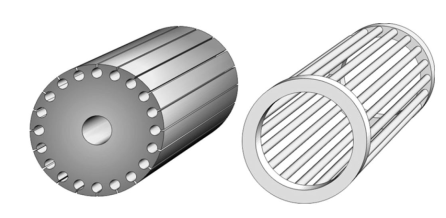
\includegraphics[width = 4.5in]{./Figures/MS/27.png}
		\rule{35em}{0.5pt}
	\caption{Laminated core(left) and steel structure(right)}
	\label{fig:Laminated core(left) and steel structure(right)}
\end{figure}

This sort of cage is next positioned inside a laminated core to reduce magnetic leakage and eddy current losses. Outer assembly of this laminated rotor core is shown on the left in Figure 2. Additionally, the conduction bars are typically not positioned entirely parallel to the orientation of the shaft, as shown in Figure 2, but slightly tilted. This practice is called skewing and it reduces cogging effect that might cause a blocked rotor situation. Additionally, this method minimizes the magnetic hum and sound produced by the motor. The illustrated rotor assembly is the most used in the field. However, altered variants as regards to the shape and size of the bars are used. Occasionally, even a double-cage rotor is used to achieve desired features. 

The other key element is the stator winding. Induction motor stator comprises wound coils. These are mostly made of ring-shaped copper wires or moulded flat copper structures. The coils are positioned in a laminated assembly as the cage rotor to avoid eddy current losses and to minimize magnetic leakage. Together, the rotor and the stator formulate a magnetic circuit. A rotating magnetic field is formed in the air gap between the stator and the rotor when a sinusoidal voltage is applied. The rotational speed of the magnetic field is called synchronous speed and defined as:
\begin{equation}
	n_s=(120*f_s)/p
\end{equation}
\begin{align*}
	\text{where:}\quad
	 f    &=  \text{frequency of applied voltage.} \\
	 p    &=  \text{number of poles.} \\
\end{align*}
A voltage is induced in the rotor bars according to the Faraday's law of induction due to this rotating magnetic field. Current begins to flow through the bars as they are shorted with shorting rings at both ends. Thus, creating a magnetic field in the rotor bars. However, a difference in the two magnetic fields is produced as the rotor sinusoidal current lags the stator current. This induces torque to the rotor bars causing rotational motion of the shaft.
The produced torque is proportional to the relative speed of the stator and rotor magnetic fields. In the absence of a difference, a stationary magnetic field is experienced by the rotor bars, and so, by Faraday’s law, no voltage will be induced, and hence, no torque is produced. So induction motors can never run at the synchronous speeds. This difference between synchronous speed and rotor speed si called slip and is defined as:
\begin{equation}
	s=(n_s-n_r)/n_s
\end{equation}
\begin{align*}
	\text{where:}\quad
	 n_s    &=  \text{synchronous speed.} \\
	 n_r    &=  \text{speed of rotor.} \\
\end{align*}

\subsection{Induction motor model in simulink}
The induction motor model in simulink, used for this project is taken from Electromechanical Systems, Electric Machines, and Applied Mechatronics by  S.E. Lyshevski\cite{lyshevski2018electromechanical}. It uses the following differential equations:
\begin{figure}[!htbp]
	\centering
		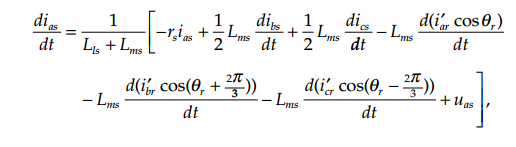
\includegraphics[width = 4.5in]{./Figures/MS/eq23.png}
		\rule{35em}{0.5pt}
\end{figure}
\begin{figure}[!htbp]
	\centering
		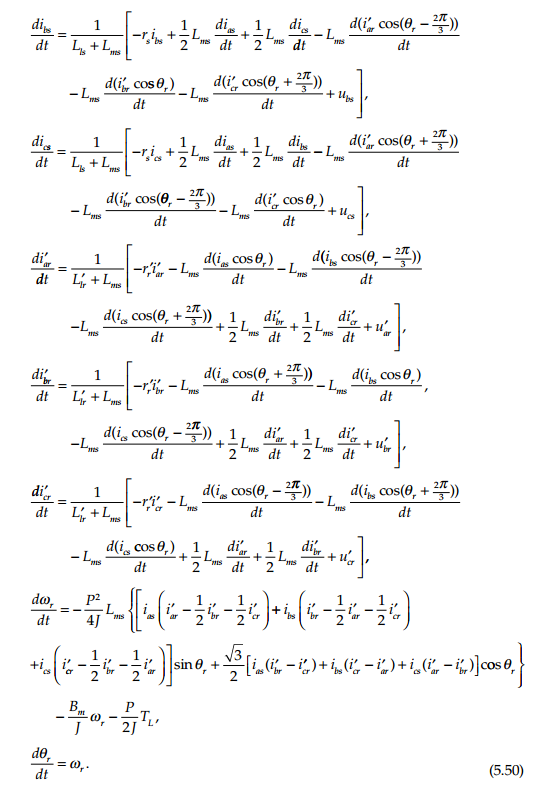
\includegraphics[width = 4.5in]{./Figures/MS/eq24.png}
		\rule{35em}{0.5pt}
\end{figure}

\clearpage
And the following model is developed:
\begin{figure}[htbp]
	\centering
		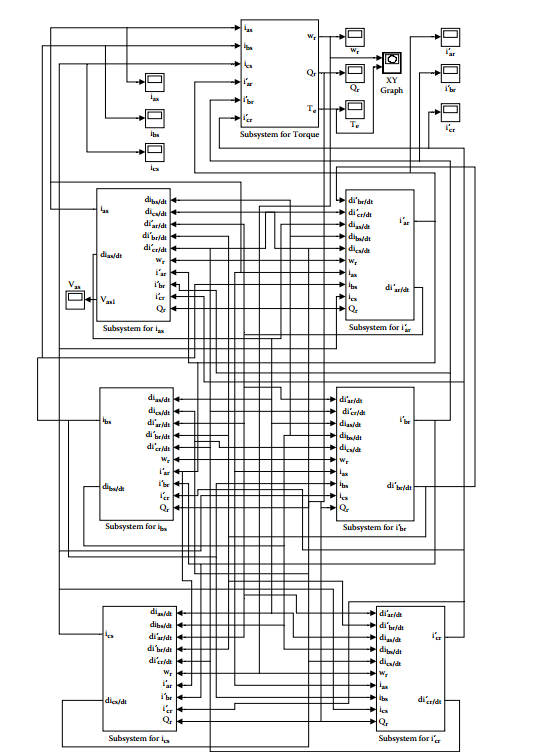
\includegraphics[width = 4.5in]{./Figures/MS/eq28.png}
		\rule{35em}{0.5pt}
	\caption{Block view of simulink induction motor model}
	\label{fig:Block view of simulink induction motor model}
\end{figure}

\clearpage
\section{Types of Losses}
According to the IEC standards\cite{iec6003421}, following are the types of losses in induction motors:
\begin{itemize}
\item Constant Losses
\subitem Iron(core) Losses
\subitem Friction Losses
\subitem Windage losses
\item Variable losses
\subitem Stator Copper(winding) losses
\subitem Rotor Copper(winding) losses
\subitem Stray or Additional load losses 
\end{itemize}

\begin{figure}[htbp]
	\centering
		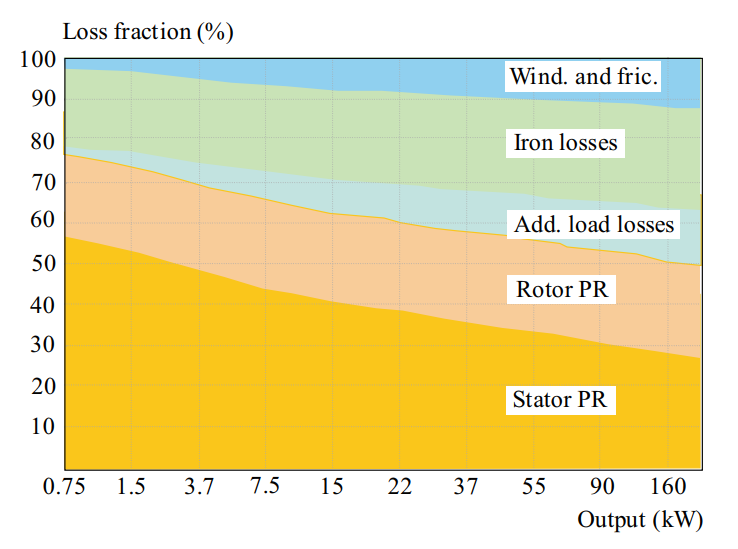
\includegraphics[width = 4.5in]{./Figures/MS/21.png}
		\rule{35em}{0.5pt}
	\caption{Typical loss distribution in induction motors}
	\label{fig:Typical loss distribution in induction motors}
\end{figure}

\subsection{Iron losses}
These are the losses in the active iron and additional no-load losses in other parts. They are divided into two losses:
-	Eddy current losses
-	Hysteresis losses
The eddy current losses are produced due to current flowing in the magnetic core, while hysteresis losses occur due to magnetization and demagnetization of the electromagnet.

Eddy current loss can be given by:
\begin{equation}
P_e=K_e * (B_max)^2 * f^2 * t^2 * V
\end{equation}
\begin{align*}
\text{where:}\quad
 K_e    &=  \text{eddy current constant.} \\
 B_{max}    &=  \text{flux density (Wb/m\textsuperscript{2}).} \\
 f    &=  \text{frequency .} \\
 t    &=  \text{material thickness.} \\
 V    &=  \text{volume.} \\
\end{align*}
So, eddy current loss mainly depends on the frequency and dimensions.

Hysteresis loss is given as:
\begin{equation}
P_b= \eta * (B_max)^n * V
\end{equation}
\begin{align*}
\text{where:}\quad
 \eta    &=  \text{Steinmetz hysteresis coefficient, depending on material .} \\
 B_{max}    &=  \text{flux density (Wb/m\textsuperscript{2}).} \\
 t    &=  \text{Steinmetz exponent, ranges from 1.5 to 2.5, depending on material.} \\
 f    &=  \text{frequency .} \\
 V    &=  \text{volume.} \\
\end{align*}
So hysteresis loss also depends on the frequency and dimensions.

\subsection{Friction Losses}
These are the losses due to friction in bearings, brushes, etc. and don't include any losses from separate lubricating systems.

\subsection{Windage Losses}
Theses are the losses due to aerodynamic friction in all parts of machine, including shaft mounted fans, etc.

\subsection{Winding or Copper Losses}
The I\textsuperscript{2}.R losses are known as copper losses or winding losses. These occur in the rotor and the stator. Their measurement is simple in case of stator, while for rotor, these are calculated using separation of losses method as it is not directly measurable.

\subsection{Additional Load Losses}
These are miscellaneous losses due to stray flux when machine is loaded, eddy current losses in winding conductors caused by load current dependent flux pulsations and additional brush losses caused by commutation, etc.

\section{Factors contributing towards motor efficiency}
Following are the factors mainly contributing towards a motor's efficiency\cite{manoharan2009review}:

\subsection{Active Material}
The active material is the main material in the motor that is responsible for electromechanical conversion. It is mostly copper or aluminium. The motor efficiency can be increased by increasing the active material, but this needs to be optimized for cost and weight.

\subsection{Lamination materials}
Instead of using a large block of iron as core, laminated thin sheets of iron are used to drastically reduce the eddy losses. High performacnce lamination materials(permeability, losses, and insulation)  can be used  to improve the efficiency further 

\subsection{Temperature levels of motor}
The stator and rotor I\textsuperscript{2}.R losses are directly proportional to the motor temperature levels. By designing the motor for better heat flow and heat transfer from active to non-active parts, the temperatures can be lowered, hence improving the efficiency.

\subsection{Stator and rotor geometries}
With careful optimization of stator and rotor geometries, the motor efficiency can be greatly enhanced. A non symmetric design will be prone to vibrations due to unbalancing, etc.

\subsection{Air gap dimensions}
Air gap dimensions are likewise an important item to be optimized to achieve improved efficiency without essentially increasing the overall material cost.

\subsection{Manufacturing Processes}
Optimization of manufacturing procedures is the one of the important factors to reduce stray-load losses, which are hard to foresee and, in general, merely to be determined by 
prototype testing

\subsection{Fan efficiency}
An efficient fan can help reduce friction and windage losses.

\subsection{Bearing efficiency}
By reducing the bearing friction, we can gain a small amount of improvement in efficiency.

\begin{figure}[htbp]
	\centering
		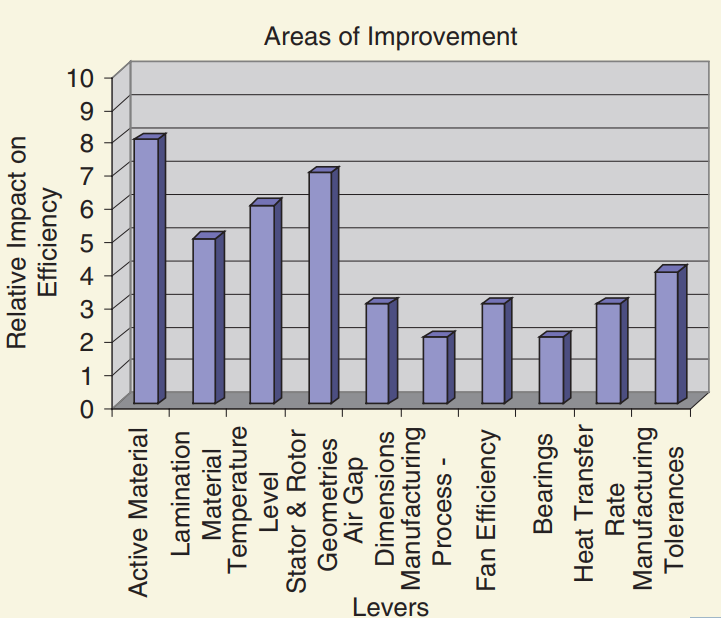
\includegraphics[width = 4.5in]{./Figures/MS/22.png}
		\rule{35em}{0.5pt}
	\caption{Impact of possible areas of improvement on efficiency}
	\label{fig:Typical loss distribution in induction motors}
\end{figure}

\section{Machine Testing methods}
Machine testing can be divided into two main types:
\begin{itemize}
	\item Direct testing
	\item In-direct testing
\end{itemize}

\subsection{Direct Testing}
In direct testing, the motor is put to full load and all the quantities e.g. speed, torque, voltage, current, etc are measured directly, and the whole power developed is wasted. Examples include brake testing. Direct testing can only be done for small machines.

\subsection{In-direct Testing}
These methods consist of measuring the losses and then calculating the efficiency. The simplest of the indirect test is Swinburne’s test. Hopkinson test is commonly used test under this method on shunt motors. These methods are also beneficial when the motor is installed in field and cannot be removed. Other examples include nameplate method, slip method, current method, statistical method, equivalent circuit method, segregated loss method, air gap torque method, and shaft torque method. The slip and current and other such methods use nameplate data while the equivalent circuit method requires a knowledge of the machine parameters such as inductances, resistances and calculates the motor operating conditions using state space models, etc. and is used in mathematical techniques such as deep learning, etc.

\subsection{Methods defined in the IEC method}
The IEC standard has defined multiple methods for testing which include both direct and indirect methods. The direct methods are defined in the preferred testing methods section, while the indirect methods are defined in the routine/field testing methods.

\begin{figure}[htbp]
	\centering
		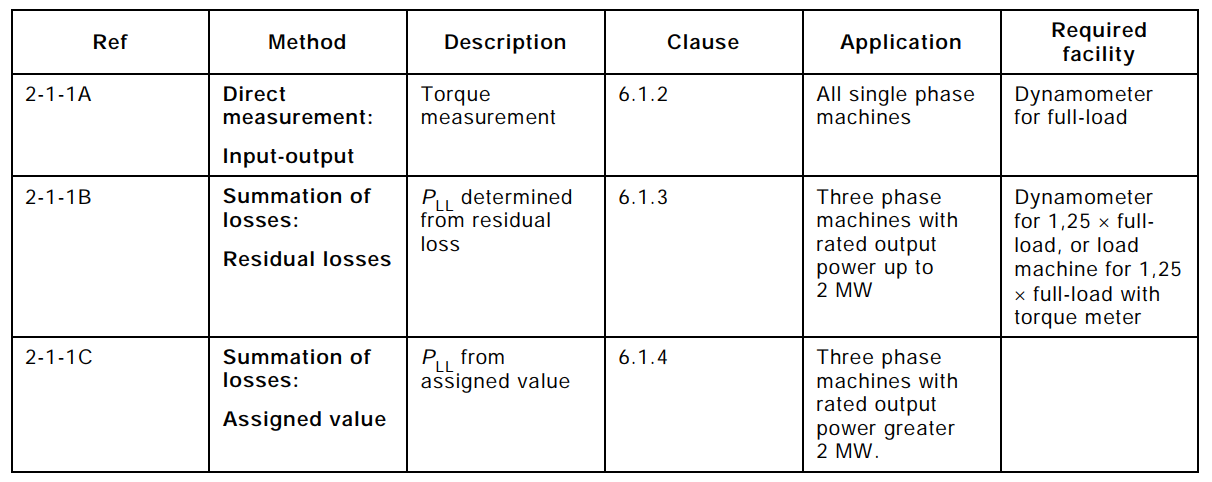
\includegraphics[width = 5.5in]{./Figures/MS/23.png}
		\rule{35em}{0.5pt}
	\caption{Preferred testing methods defined by IEC 60034-2-1:2014}
	\label{fig:Preferred testing methods defined by IEC 60034-2-1:2014}
\end{figure}
\begin{figure}[htbp]
	\centering
		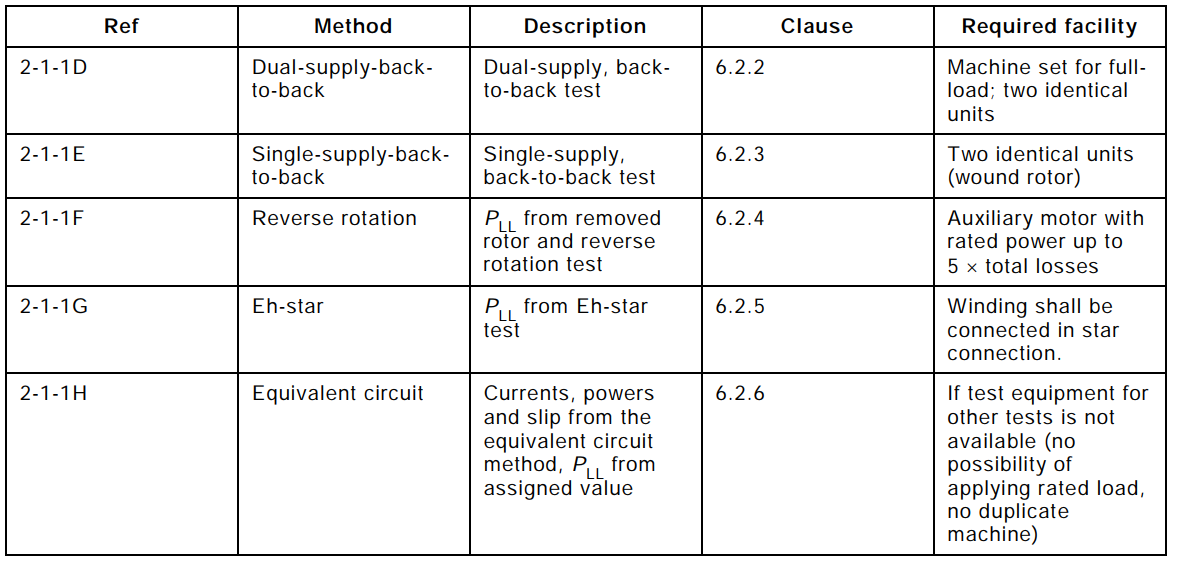
\includegraphics[width = 5.5in]{./Figures/MS/24.png}
		\rule{35em}{0.5pt}
	\caption{Routine/Field testing methods defined by IEC 60034-2-1:2014}
	\label{fig:Routine/Field testing methods defined by IEC 60034-2-1:2014}
\end{figure}

\subsection{Testing methods with pumps}
Testing of pumps is done under ISO-9906\cite{iso9906} standard which provides conditions and requirements for testing of pumps. The following table shows the accuracy of pump testing:
\begin{figure}[htbp]
	\centering
		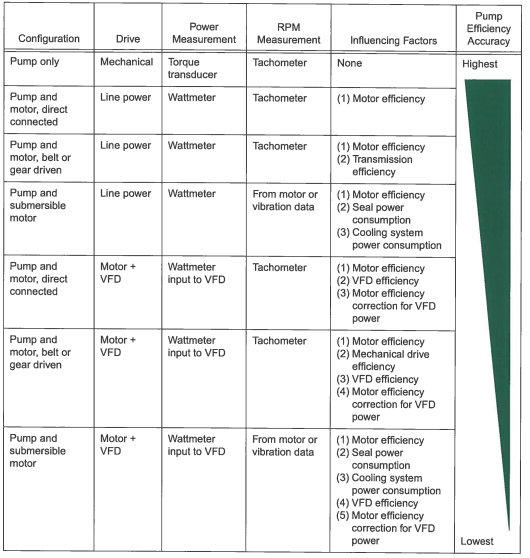
\includegraphics[width = 5.5in]{./Figures/MS/25.png}
		\rule{35em}{0.5pt}
	\caption{Testing Accuracy by configuration defined by ISO-9906}
	\label{fig:Testing Accuracy by configuration defined by ISO-9906}
\end{figure}
This table shows that the best accuracy is achieved in the case of separate testing of pumps and motors. So, IEC 60034-2-1 was used for testing the motors separately.